\chapter{词向量的构建}

\section{词向量在本课题中的研究背景}


如第一章分析,要能够实现基于人类做的自然语言到色彩的自动转化, 这首先是要进行文本涵义的表征。 需要将日常的文字变换成计算机能够读懂的数字化或者向量化的表征方式。 对于一句话的表征, 即前文中所叙述的sentence embedding -- 句向量嵌入 -- 是目前基于自然语言应用的重要步骤。 句子的嵌入化操作, 能够使得一句话变成计算机能够直接进行计算的向量。  而要进行句子的向量化, 目前常见的方式是基于“单词”进行, 因为“单词”是能够表征文字信息的最小单位。 我们先对单词进行向量化, 这种向量化为之后的句子的向量化提供了基础, 从而为句子的“语义”级别的理解提供了可能。 

由于单词的向量化是长久以来一直研究的问题, 其方法众多,而且单词的向量化在2014年之后, 由于Google科学家Micolve想提出的向量化方法, 众多的科研工作者们在此领域有了长足的发展。 本章首先阐述单词向量化的必要性, 以及解释目前单词向化不同方法的优劣, 从而提出一种适用于本课题的单词向量化方法。 

\section{单词向量化的必要性}

要使得计算机具有能够识别语言的能力, 计算机机需要能够在某种层面上计算语言的相似性,即,输入两个语义单元,计算机需要能够判断其相似关系。 例如, 输入“喜欢”和“爱”,由计算机给出的相似性应该要小于“喜欢”和“讨厌”之间的距离。 即, 计算机应该具有某种函数 $Sim()$, 该函数接受两个单词的输入$R_{w1}, R_{w2}$, 输出正则化的 $ -1 ~ 1$ 用以表示两个单词的意思从“很不相思”/“相反”到“很相似”。 

$$ Sim(R_{w1}, R_{w2}) \in [-1, +1] $$

如果计算机能够计算这种相似性,那么接下来的句子、段落等更高层面的语义相似性计算机便成为了可能。 而要让计算机具有这种能力, 首先需要考虑的就是如何表示单词$w1, w2$。 

我们可以给单词标号, 假设目前有$|V|$个单词, 那么依照某种顺序, 例如“字典序”对每个单词进行标号, 然后依据字典或其他某种方式定义出来每个单词的近反义词, 然后计算单词相似度的时候, 检查任意两个单词是否为近义词或者反义词即可。 

```
	vocabulary = {
		0: {
			'word': '爱恋', 	
			'syn': '喜爱', '喜欢', '喜爱',
			'ant': '讨厌', '憎恨'
		   }
		1: {
			 'word': '苹果', 
			 'syn': '水果', 'apple',
			 'ant': ''
			}
	}
```

以上的表示方式是长久以来计算机表示单词的方式, 在这种实现方式下, 能够较为“基础”的实现单词的近反义词的判断。 但是这种表示存在3个问题: 

\begin{enumerate}
\item{\textbf{人工整理成本高}}:该种表示方法, 首先需要人工进行同反义词的输入,而人工整理输入就面临着成本高, 容易出错等问题;
\item{\textbf{不能动态适配不同的语料}}:该种表示方法,对于不同的语料库,不能把握其近反义词。 例如,对于一个科技类资料库的文本库, “苹果”的近义词应该是“IBM”,“微软”, 但是对于生物类的文本库, “苹果”的近义词应该是“梨子”。 

\item{\textbf{不能精确衡量相似度}}: 该种表示方法,对于任意两个单词, 其内在逻辑是判断这两个单词是否为“近义词”或者“反义词”,输出为一个离散值 $Output \in {Syn, Ant,None}$, 但是用这种离散的方式表示单词关系是不能蕴含词汇之间丰富的关系的。 例如, “美国”和“奥巴马”之间, 这两个单词之间既不是“相似”单词,也不是“不相似”单词, 但是更不是“没有关系”的单词。 

\end{enumerate}

由于以上存在的问题, 是的我们必须考虑使用新的单词表示方法,该单词的表示方法需要满足以下条件::

\begin{enumerate}

\item{计算机能够计算}: 该表示首先需要让计算机能够计算, 让计算机能够计算, 则需要将其表示成数字(标量或者向量)的形式, 我们在这里可以将标量看成是一维的向量, 所以下文统称为 \textbf{向量};

\item{能够计算单词之间的相关性}: 利用单词的向量表征,能够计算不同单词之间的相关性, 该相关性应该为从 -1 到 1 的连续值。 

\item{能够自动化适配于不同的语料库}: 该向量化方式应该能动态适配与不同的语料库, 竟可能少的需要人工参与。 

\end{enumerate}

\section{单词向量化的基本原理}


单词(或者文本)的向量化在2014年之前主要使用TF-IDF这种依赖单词概率分布的向量形式进行表示; 而对于单个单词主要使用one-hot编码进行。

\subparagraph{one-hot编码}
one-hot 编码基于上文提到的标号编码的一种向量表示, 这两种其实本质是一样的,都是将每个单词表示为唯一的类型(categorical)。如表 \ref{table:one-hot} 所表示\cite{athier1997process}我, 例如一句话:“我 喜欢 吃 苹果,而 他 喜欢 吃 梨子。”这个句子长度为7个不同的单词。我们可以用这样的向量给每个单词编码,每个单词就可以表现为一个7维的向量,如表~\ref{table:one-hot},每个单词的向量为单词下的一列,就可以将一段文本的信息完整的保存进一个矩阵。

\begin{table}[!htbp]
\caption{one-hot向量}
\label{table:one-hot}
\centering
\begin{tabular}{|c|c|c|c|c|c|c|c|c|c|}
\hline
  & 我 & 喜欢 & 吃 & 苹果 & 而 & 他 & 喜欢 & 吃 & 梨子 \\
\hline
我 & 1 & 0 & 0 & 0 & 0 & 0 & 0 & 0 & 0 \\
\hline
喜欢 & 0 & 1 & 0 & 0 & 0 & 0 & 0 & 0 & 0 \\
\hline
吃 & 0 & 0 & 1 & 0 & 0 & 0 & 0 & 0 & 0 \\
\hline
… &  &  &  &  &  &  &  &  &  \\
\hline
\end{tabular}
\end{table}

这样的方法, 不可避免的有以下问题:

\begin{itemize}

\item{存错空间消耗大}: 如果对于文本长度较大的情况,就需要很大的空间储存这些向量,比如一本上万个单词的书籍,就需要单词的维度上万,里面大多数的位置又都是0;
\item{不同的语料库中,同样的单词表示不同}: 这种方式对于不同文本来说并没有同一性,对于同一个词,不同的文本中必须有不同的词向量;
\item{单词表征无法保持语义的相似性}: 这些词向量很难表示词的含义,因为, 任意两个向量 $\vec{v_1},  \vec{v_2}$ 的单词向量距离都是相等的, 都是 $\sqrt{2}$

\end{itemize}

\begin{table}[!htbp]
\caption{词频向量}
\label{table:frequency-vec}
\centering
\begin{tabular}{|c|c|c|c|c|c|c|c|}
\hline
句子 & 我 & 喜欢 & 吃 & 苹果 & 而 & 他 & 梨子 \\
\hline
我喜欢吃苹果而他喜欢吃梨子 & 1 & 2 & 2 & 1 & 1 & 1 & 1 \\
\hline
我喜欢吃苹果,梨子 & 1 & 1 & 1 & 1 & 0 & 0 & 1 \\
\hline
他喜欢吃吃吃 & 0 & 1 & 3 & 0 & 0 & 1 & 0 \\
\hline
\end{tabular}
\end{table}

\subparagraph{tf-idf词频编码}

为了减少向量的维度,增加矩阵的密集程度,出现了基于词频的单词向量化。以我们的例句为例“喜欢”,“吃”这两个单词出现了两次,其他单词出现了一次。词频向量就是基于此构成。如表~\ref{table:frequency-vec},例如一篇文章中有表中的三句话,则每个单词的向量为单词下的一列,每句的向量为句子右侧的一行。词频向量和one-hot向量相比,维度有所下降,使用空间更有效率。词频也会记录一些文本的信息,不同的文本中单词的词频会有区别。然而完全从句子对单词计数,对词序信息完全忽略,同样难以提取文字本身的含义。

在此基础上的tf-idf的向量化不仅仅量化一个单词在一段文本中的频率,还考虑到在所有文本中单词出现的情况,这样就可以表征出一个单词和某段文本的关系。\cite{xia2011improvement}$tfidf = tf(t,d)*idf(t,D)$,其中 $tf(t,d)$ (term frequency)表征单词t出现在文本d中的频率。它可以有多种形式,比如$tf(t,d)=f_td$,$f_td$表示单词t出现在文本d中次数;或者考虑到文本到长度$tf(t,d)= \frac{f_td}{n_{in document}}$,$n_{in document}$指文章总共的单词数,$tf(t,d)$即出现在文本中的频率;甚至也可以是布尔的,当文本d中出现词t则 $tf(t,d)=1$ 否则$tf(t,d)=0$,等等。idf(inverse document frequency)定义为$idf(t,D) = log\frac{N}{n_{t occurs}}$ ,$N$表示总的文档数,$n_{t occurs}$表示含有单词t的文档数。

以之前的三句话为例:(a)我 喜欢 吃 苹果 而 他 喜欢 吃 梨子。(b)我 喜欢 吃 苹果。(c)我 喜欢 吃 吃 吃。则对于单词“我”,有:$tf(“I”,a)= \frac{1}{9}$,$tf(“I”,b)= \frac{1}{4}$,那么句子b中“我”这个词占整体比例更高。但对于所有文本,$idf(“I”,D) = log\frac{3}{3} = 0$,每个句子都出现了“我”这个词,所以$tfidf(“I”,a) = tfidf(“I”,b) = 0$。处理文档大量时,对于一些非常常见的词,比如“那个”“这个”这样的词,可以认为它们没什么意义,就会出现这种情况。而比如对于单词“苹果”,$tf(“apple”,a)= \frac{1}{9}$,$tf(“apple”,b)= \frac{1}{4}$,$idf(“apple”,D) = log\frac{3}{2} $,就会出现$tfidf(“apple”,a) = 0.045$,$tfidf(“apple”,b) = 0.1$。我以这三个句子计算了单词“我”和单词“苹果”的向量如表~\ref{table:tfidf-vec}:

\begin{table}[!htbp]
\caption{tfidf向量}
\label{table:tfidf-vec}
\centering
\begin{tabular}{|c|c|c|c|}
\hline
句子 & 我喜欢吃苹果而他喜欢吃梨子 & 我喜欢吃苹果 & 我喜欢吃吃吃  \\
\hline
我 & 0 & 0 & 0  \\
\hline
苹果 & 0.045 & 0.1 & 0 \\
\hline
… &  &  &  \\
\hline
\end{tabular}
\end{table}

tf-idf向量的表示可以从一定程度上衡量不同句子、文本之间的相似性, 但是tfidf显然还是不能处理同义词和近义词的问题。 例如“我早晨去上班”和“我清晨要去打卡”, 这两句话的意思其实是很相似的, 但是对于tfidf向量化来说, 对于词表 [“我”, “早上”, “清晨”, “要去”, “去”, “上班”, “打卡”], 第一句话 “我早晨去上班”会得到向量 <a, b, 0, 0, c, d, 0> 而 第二句话的向量为 <e, 0, f, g, 0, 0, h>, 这两句话的向量距离为 $sqrt{(a-e)^2 + (b-0)^2 + (f-0)^2 + (g-0)^2 .. + (0 - h) ^ 2}$, 这是一个相对比较大的距离。 利用tfidf表示, 这两句话计算机只能发现“我”和“我”的意思是一样的, 但是对于其他不一样的单词, 虽然是同义词或者近义词, 但是计算机依照这种表示方式, 依然会认为是完全不一样的单词,从而不能表示其相似性。 

\section{word2vec单词向量化}

如上文所述,利用one-hot或者tfidf向量化能够完成使计算机进行计算的问题,但是存在以下比较显著的问题: 

\begin{enumerate}
\item{不能识别近义词,同义词}:不论是one-hot还是tfidf表示,都不能表示近反义词等,而能自动识别近反义词, 同义词其实是语言理解中很重要的一个环节, 因为只有这样,才有可能完成不基于单纯的“关键词”匹配完成语言分析。 
\item{需要很大的存储空间}: one-hot和tfidf存储的都是稀疏向量,需要很大的存储空间;
\item{不能适应性更新 (Adaptive Updating)}: 该问题值得是, 如何我们已经有了10000个单词的one-hot词向量编码或者10000句话的句子tfidf编码, 基于one-hot和tfidf的原理, 如果我们新增加了100个单词或者句子, 我们需要把这10000 + 100个句子全部更新。 这显然是不合理的。 因为如果每次增加新的数据都要对全部的数据进行更新, 那么当已经存储的数据量很大的时候, 每一次增加新词汇、新句子的成本就会很大。 
\end{enumerate}

2013年Google的科学家Mikolov在《Efficient Estimation of Word Representations in Vector Space》\cite{Mikolov:2013:DRW:2999792.2999959}中提出的基于神经网络的非监督词向量构建方法,获得良好的结果, 在2014年, 在此基础之上有提出了Negative Sampling, Hirerachy Softmax等优方法,使得该种词向量的计算效率大大提升。

从2014年到2017年,基于word2vec的词向量表征领域的进步显著, 在2014年由Stanford NLP Group 提出的GloVe, 2016年提出的Fasttext, 2017年salesfore提出的CoVe (Context Vector), 直到2018年提出的EMLo(Embedding from Language Model)使得单词的向量表征获得很大的提升。 基于词向量的成功,推动了自然语言理解领域多个子领域的进步, 其中包括: 1. 语言相似判断; 2. 机器阅读理解; 3. 文本匹配; 4. 蕴含识别。

因此, 本课题的单词训练方法也采用word2vec的思想, 但是由于本课题所面临数据库的特殊性, 需要在原始的word2vec算法上做一定的修改。 本小节首先描述word2vec的基本原理。 


word2vec是Mikolov提出的一种将单词进行向量化的方法。 该向量化方法主要基于语言学家 J.R.Firth 在1957年提示的理论,“You shall know a word by the company it keeps”, 即在语言学中认为,一个单词的意思可以通过其单词周围的单词的来进行判断。在英语考试里边的“完型填空”, 我们通过判断周围的单词就可以判断某个缺失的地方应该填入什么单词。 例如, 如果我们的观察 “到了春天, 这里的竹笋[ ]得很好”, “这条河两个岸边距离很远, 需要建一座很[ ]的桥”。我们可以知道这两句话里边都是要填“长”这个词, 但是这两句话里边的“长”字的意思又是不一样的。 这表明了一个单词其实依据它周围的词就可以确定出来。 

word2vec基于这种假设, 希望能够利用一个单词与其周围单词的关系来确定单词的词向量。 其基本思路为, 每一个单词都有一个初始的随机向量表示,该向量表示可以是几十到几百维度的向量。 我们将单词进行标号, 假设其标号为 $i$, 那么, 单词 $i$ 的向量表示为 $\vec{w_i}$, 如何确定这个单词? 

wordvec提出了两种方法, 一种是skip-gram, 一种是CBOW。 其中, skip-gram设计一个机器学习模型,该模型的目标为输入一个单词的词向量 $\vec{w_i}$, 对此词向量进行线性变化, 之后将该单词进行 $softmax$ 函数变化, 使得依据该单词向量,能够求得该单词周围出现的单词。 即, skip-gram希望拟合这样一个模型,公式 \ref{eq:skip-gram-model}, 该模型通过输入单词的词向量 $\vec{w_i}$, 能够预测其周围应该分布什么单词。 

\begin{equation} 
Y(\vec{w_i}; \theta) = w_i,  w_i \in context_i
\end{equation}
%model(\vec{w_i}; \theta) = {w_j, w_k, w_l}, w_j, w_k, w_l \in \mathbb{V}

skip-gram基于一批训练数据,该训练数据为数据量较大的文本信息。 skip-gram每次指定一个单词,然后训练该模型, 使得模型能够预测周围单词的分布,该模型输入一个单词的向量, 依据此向量产生的周围单词的分布为 \ref{eq:skip-gram-loss}: 

\begin{equation} \label{eq:skip-gram-loss}
Pr(\vec{V_o} | \vec{V_c} ; \theta ) = \frac{e^{ \vec{V_o}^t \cdot \vec{V_c}}}{\sum_{i \in \mathbf{V}}{e^{v_i^t \cdot v_c}}}
\end{equation}

获得了周围单词分布的概率估计,就可以使用神经网络的交叉熵(cross entropy)方式进行反向传播(back propagation), 值得指出的是, word2vec模型(包括skip-gram与CBOW)与普通的神经网络模型并不完全一样。 因为,普通的神经网络模型其反向传播之后,利用随机梯度下降(SGD)等方式是对参数集 $\theta$ 进行更新, 对于输入的$X$值,并不更新。但是 word2vec 与其他神经网络模型不同的是,word2vec的反向传播模型会一直延续到输入值$X$, 也就是说, 其每一次的输入 $V_c$ 的向量, 也是会通过反向传播的方式进行更新的。 在每一轮(epoch)的更新中, 每个单词的向量会得到更新, 而这种更新的结果就是, \textbf{如果两个单词周围经常出现的单词比较相似,那么这两个单词的词向量也会比较相似}。 word2vec模型简单高效容易操作, 获得的词向量结果能够良好的保持语言的相似性。 例如基于中文维基百科进行word2vec的训练,我们可以获得如图 \ref{img:word2vec-math} 的近义词关系。 

其中图 \ref{img:word2vec_math} 一共表现了word2vec的四种重要的特性: 

\begin{enumerate}
\item{\textbf{同义词近义词发掘}}: 例如当输入“数学”的时候, 我们可以获得与“数学”单词涵义接近或者类似的单词;
\item{\textbf{单词线性关系的保持}}: 保持线性关系这个特性是word2vec模型最为突出的一有点, 例如对于单词“女人”和“妈妈”的向量, 这两个单词之间的距离最近解决与“男人”和“爸爸”之间的距离。 这表明了word2vec模型精确得定义了单词之间的语言距离。 
\item{\textbf{同一类型单词的自动识别}}: word2vec因为将具有关联关系的单词进行了自动聚类,所以可以识别出任意的单词是不是属于同一相关类型, 例如在图中, 能够识别“牛肉”与“黑板, 作业,老师”不属于同一个类型。
\item{\textbf{任意两个单词之间的关系计算}}: word2vec可以计算任意两个单词之间的相关关系。 
\end{enumerate}


\begin{figure}[htbp]
    \centering  % 学位论文规定图表皆水平居中于版心 在 zjuthesis.cls 搜「版心设置」
    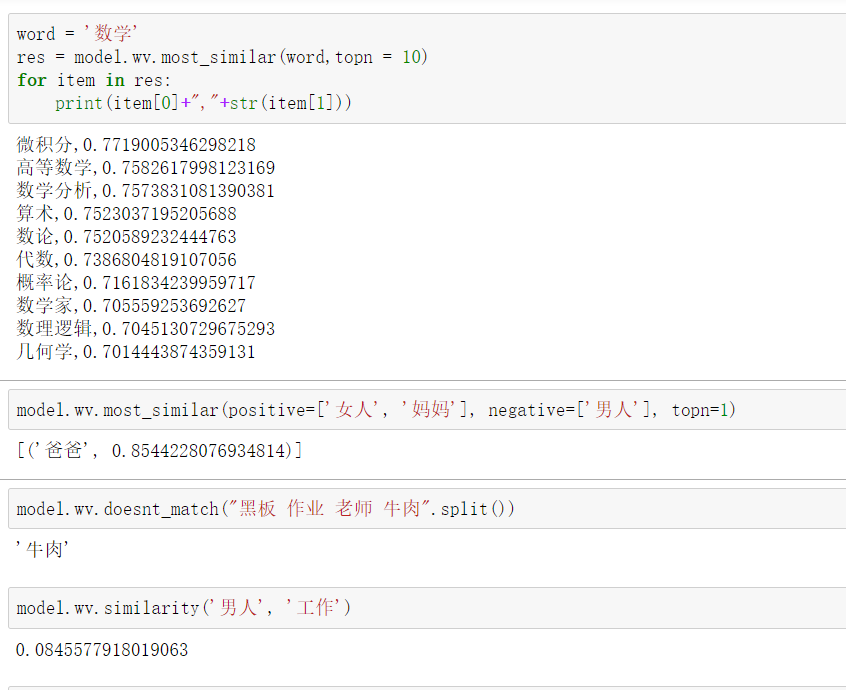
\includegraphics[width = .55\linewidth]{data/chapter-1-1/word2vec-math.png} % 设定图片宽度相对于版心宽度,图片文件资源名
    \caption{word2vec的语言相似性实例} % 图的题注
    \label{img:word2vec_math} % 与 autoref 关联,设定交叉引用和显示「图x.x」
\end{figure}

而且,利用高维向量的降维可视化TSEN,可以对训练出来的向量进行可视化。 TSEN是一种高维向量的可视化方式,该算法可是使得如果两个向量在高维空间中接近, 那么在降维之后两个向量的距离依然相近。尽管我的实际观察发现,其语义相似的单词, 经过word2vec模型训练得到的最终向量距离确实更相近。 如图 \ref{img:tsne} 所示, 和污染物相关的单词就被聚类到了相近的距离。 


\begin{figure}[htbp]
    \centering  % 学位论文规定图表皆水平居中于版心 在 zjuthesis.cls 搜「版心设置」
    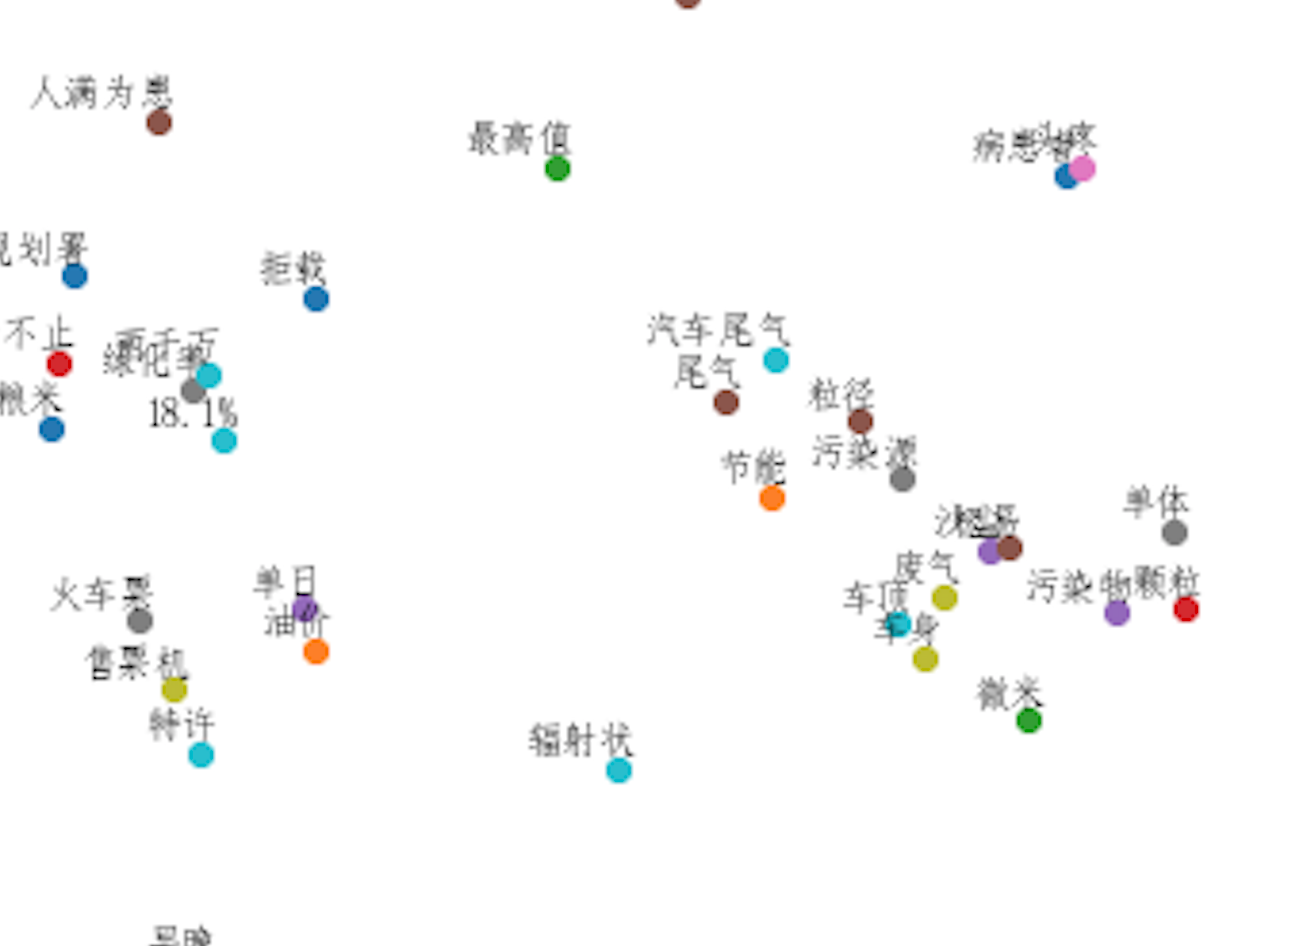
\includegraphics[width = .55\linewidth]{data/chapter-1-1/tsne.png} % 设定图片宽度相对于版心宽度,图片文件资源名
    \caption{word2vec向量聚类可视化} % 图的题注
    \label{img:tsne} % 与 autoref 关联,设定交叉引用和显示「图x.x」
\end{figure}

除了skip-gram, word2vec的方式还有CBOW(Continuous Bag of Words), 该模型与skip-grma类似,但是不同的时候, skip-gram输入的是一个单词用以预测其周围的单词, 而CBOW模型的输入是一个单词的周围单词,用来预测这些单词的“中心单词”, 例如, “我今天早上吃了一顿早饭”, skip-gram输入“早上”, 期望模型能够输出“我”, “今天”, "吃了", “一顿”, 而CBOW的输入是“我”, “今天”, “吃了”, “一顿”, 期望的输出是缺失的单词“早上”。 

初次之外, 还有Stanford NLP Group提出来的GloVe模型, 该模型用来预测两个单词同时出现的概率(co-occurance)的概率; 以及2017年和2018年提出来的CoVe(Context Vector)和ELMo(Embedding of Language Model), 这两种模型基于机器自动翻译模型的结果, 能够使得每个单词在不同的句子中的单词词向量的表征不一样, 从而更加精确的表征了单词向量。 

\section{本课题单词向量化算法的创新点与具体实现}

上文分析了单词向量化的基本原理,通过该种单词的向量化表示使得我们具有能够表征单词的能力。理论上,基于Micolvo提出来的word2vec模型, 可以实现单词的向量化。 但是由于本课题使用的数据源的限制, 利用该种word2vec模型并不能训练处有效的单词词向量, 本课题需要在已知的词向量方法上,基于word2vec的思想,设计新的模型算法,进行艺术相关词汇的词向量的训练。 

本课题使用的数据源为雅昌拍卖网艺术品交易数据库(auction.artron.net), 数据库中关于艺术品以及艺术品交易的信息丰富,包括流通的艺术品的题目、图片、特征、作者、艺术品类别、交易价格、流通时间等等。本课题所用到的数据库中的信息包括两类如图~\ref{figure:数据库结构},一类是艺术品信息,另一类为艺术品相关的文章。

\begin{figure}[!htbp]
\centering
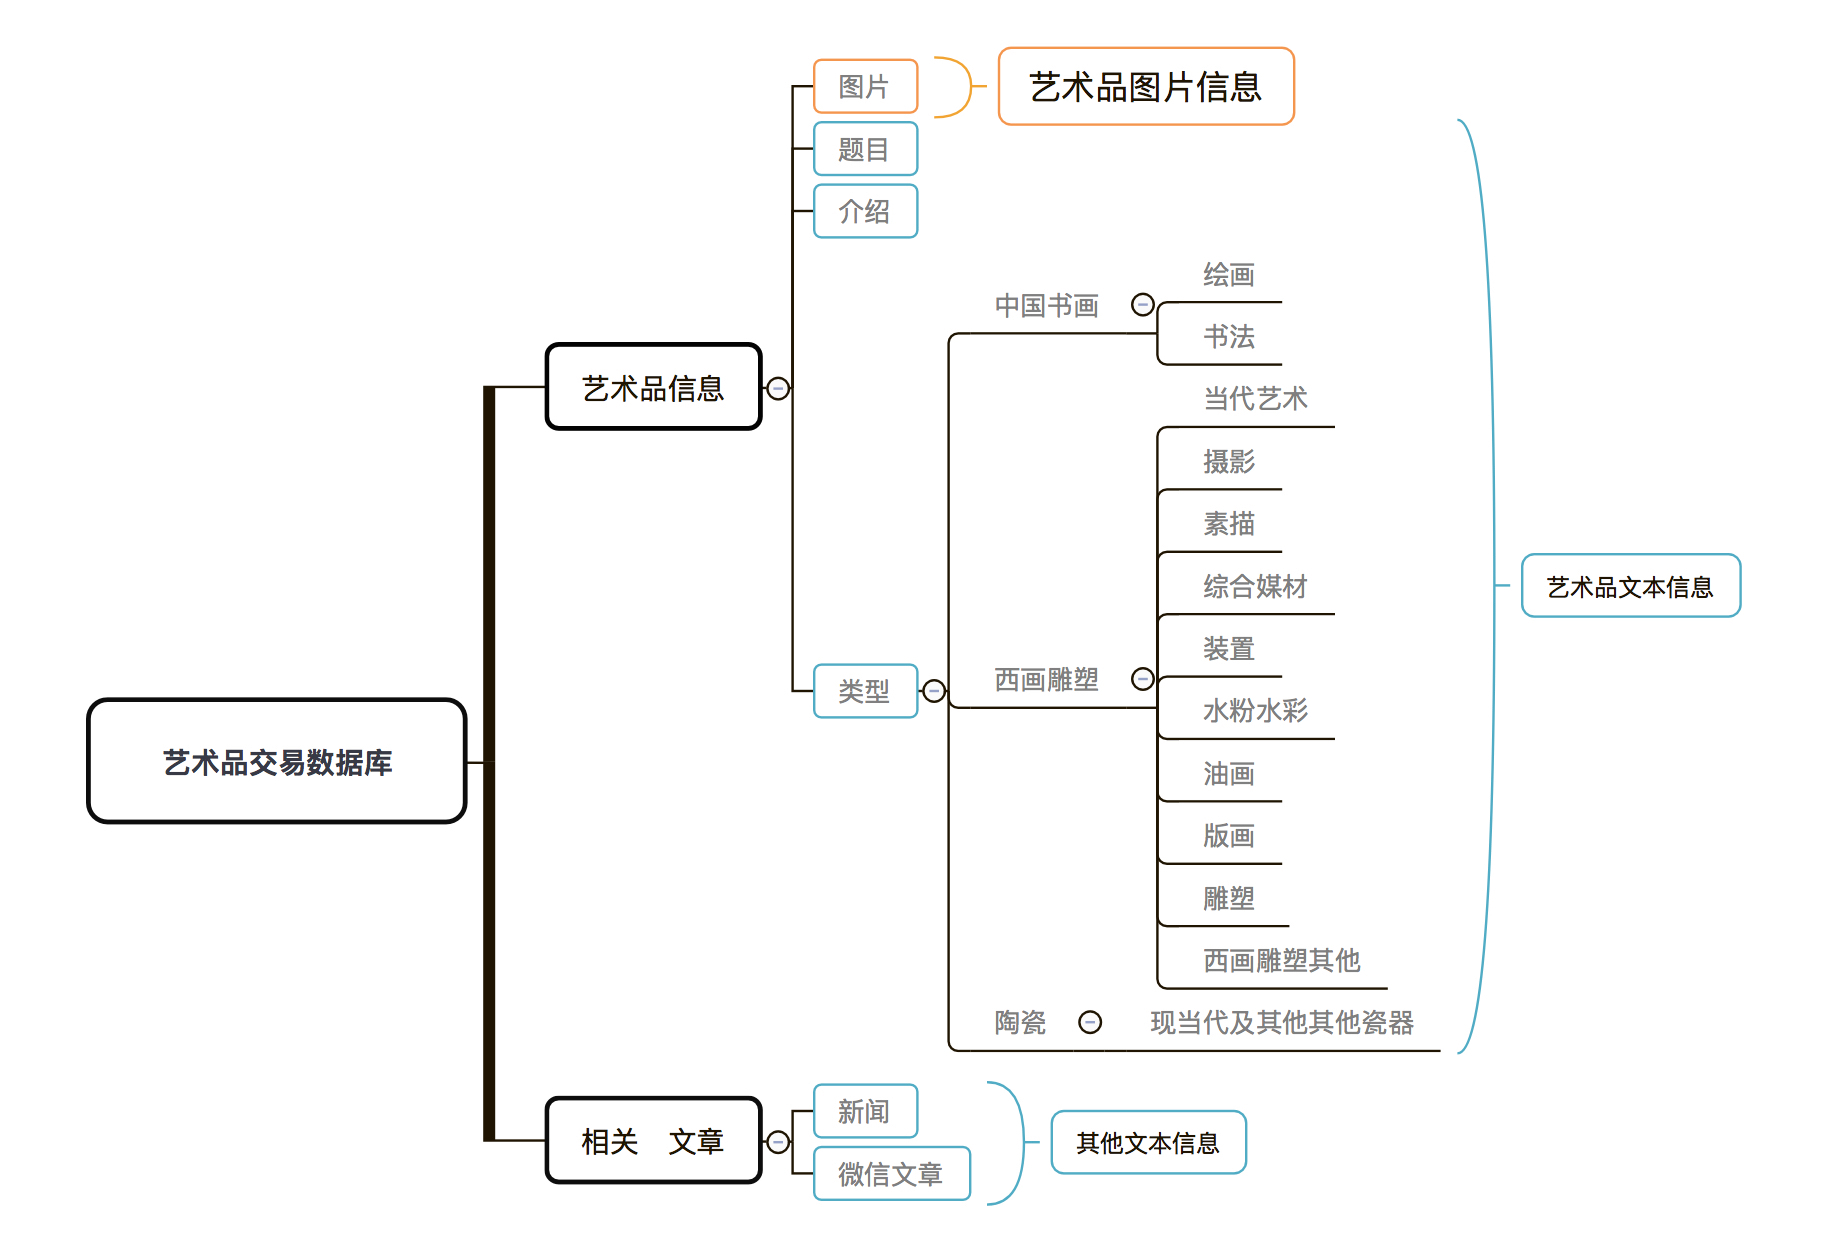
\includegraphics[width=\linewidth,keepaspectratio]{data/chapter-1/D02BCA18-F339-4988-9E23-E6C5E437BCCA.jpg}
\caption{数据库结构}
\label{figure:数据库结构}
\end{figure}

其最重要的艺术品信息的数据样例如图 \ref{figure:sample-db},该数据库比起word2vec原始模型其数据源有以下区别: 

\begin{figure}[!htbp]
\centering
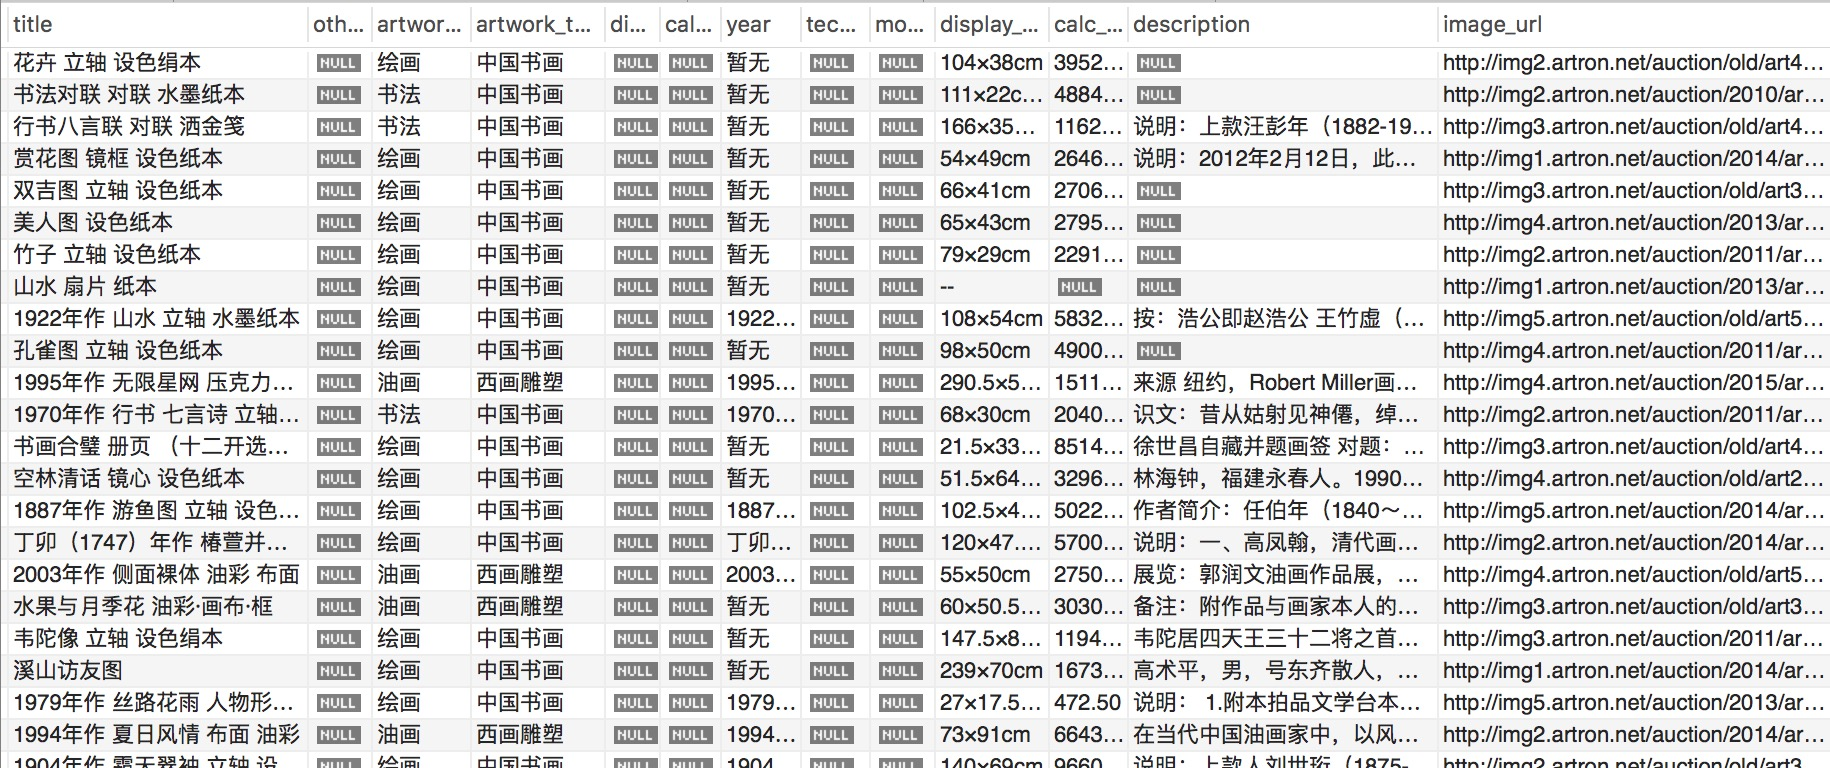
\includegraphics[width=\linewidth,keepaspectratio]{data/chapter-1-1/art-description.png}
\caption{艺术品描述信息}
\label{figure:sample-db}
\end{figure}

\begin{enumerate}
\item{\textbf{数据量小}}: 数据量较小,则会产生模型无法收敛,以至于按照word2vec的方式,不能获得有效的单词向量;
\item{\textbf{每句话较短}}: 由于每句话较短,所以有相当一部分的单词不能具有足够的上下文。 所谓上下文(context)指的是一个单词的左边和右边的N个单词, 例如“深度学习 模型 是 一种 神经网络 模型”, 那么, 当我们的上下文窗口定义为3的时候,“是”的上下文为“深度学习 模型”和“一种 神经 网络”,即, 距离在3(包括3)以内的单词都是上下文的。 但是由于每句话较短, 那么就会之后最中间的几个词汇能够获得足够的上下文, 尤其是在这句话的开头和结尾,如果我们把上下文的窗口数量定义为 $N$,那么我们期望的上下文单词应该是 $2N$。这种情况在维基百科等大语料库中是成立的, 在这种大语料库中, 绝大多数的单词在训练时候都能获得足够的上下文信息。 但是在本课题的艺术品交易数据库中,不能获得足够上下文的单词却占大多数。 

\end{enumerate}

基于以上两点的分析,本课题的词向量模型参考word2vec的原理,并且参考Stanford GloVe词向量的思想,设计了新的神经网络模型。 该模型输入两个单词,模型用以计算这两个单词出现在同一个艺术品作品的描述信息中的概率。即,训练一个模型, 该模型接受两个输入,$\vec{w_1}$ 和 $\vec{w_2}$,然后在一组参数 $\theta $ 的约束之下,预测该这两个单词出现在同一个艺术品描述信息中的概率$P$。参考前文的word2vec原理,在此模型之下,对于单词$w_1$ 和 单词 $w_2$, 如果两个单词经常出现在同一个作品的描述中,对于另外一组单词$w_1$和$w_3$也经常同时出现怎么艺术品的描述信息之中。如果<$w_1$, $w_2$>与<$w_1$, $w_3$>同时出现的概率类似,那么$\vec{w_1}$与$\vec{w_2}$输入模型, 与$\vec{w_1}$ 与 $\vec{w_3}$ 输入模型的输出结果是类似的。从而 $\vec{w_2}$与 $\vec{w_3}$ 的单词向量会收敛至相似。而基于上一节所述的word2vec的基本思想,如何两个单词经常出现在类似的位置,则这两个单词的意思也会相似。 所以, 经过以上步骤,就实现了艺术品交易单词的向量化。 

以上分析过程可以形式化的表示为, 我们需要拟合训练一个模型 $Y$, 该模型的目标函数为 \ref{eq:art_loss} 

\begin{equation}\label{eq:art_loss}
Loss(\vec{w_1}, \vec{w_2}; \theta) = -\log(\sigma(model(\vec{w_1}, \vec{w_2})))
\end{equation}

\subparagraph{数据预处理} 在训练之前,我们首先需要对数据进行预处理,本课题使用jieba分词程序进行自动化分析,而且使用隐含马尔可夫链进行新词发现。数据预处理的过程如算法 \ref{alg:preprocess}所述。 

\begin{algorithm}

\KwIn{List: A List which contains art work description information}
\KwOut{words matrix: a words matrix M, M[i][j] is the probability of $word_i$和$word_j$ co-occurrence}

\BlankLine
\emph{split each string to a words list}

$matrix\leftarrow [[]] $\;
$total-occurence \leftarrow 0$ \;

\For{$one-description \leftarrow List$}{
	\For{$word_i \leftarrow one-description$}{
		\For{$word_j \leftarrow one-description$}{
			\If{$word_j == word_i$}{$Continue$};
			$matrix[word_i][word_j] += 1$ \;
			$ total-occurence += 1$ \;
		}
	}
}

\For{$word_j \leftarrow matrix$}{
	\For{$word_i \leftarrow matrix$}{
		$matrix[word_i][word_j] /= total_occurence$ \;
	}
}

$\Return matrix$ \;

\caption{co-occurence 频率预处理}\label{alg:preprocess}
\end{algorithm}

经过算法 \ref{alg:preprocess}, 我们可以获得每个单词对之间出现在同一个艺术品描述信息之中的概率。 该概率矩阵为一个30,000 * 30,000 的矩阵, 该矩阵包含了词库中3万的词汇的同时出现的概率分布。 为之后利用神经网络进行计算提供了基础。

\subparagraph{训练神经网络} 在定义了loss函数之后,本课题建立神经网络模型进行训练。 基于之前所定义的loss函数, 该机器学习模型的输入应该为两个单词的向量,$\vec{w_1}$与$\vec{w_2}$, 然后对这两个向量进行线性计算, 将该向量映射到一维空间,再对该输出向量进行$sigmoid$函数的运算, 将其限定在 $0 ~ 1$之间, 用以表示概率。 

\begin{equation} \label{eq:pipeline}
Loss(\vec{w_1}, \vec{w_2}; \theta) = \log(sigmoid(\vec{w_1}^t \cdot \vec{w_2}))
\end{equation}

本课题是神经网络训练环境如下: 

\begin{enumerate}
\item{tensorflow 1.4}
\item{GPU GTX * 8}
\item{CPU Intel i5}
\end{enumerate}

基于tensorflow构建如图 \ref{figure:computing-graph} 所示的计算图. 

\begin{figure}[!htbp]
\centering
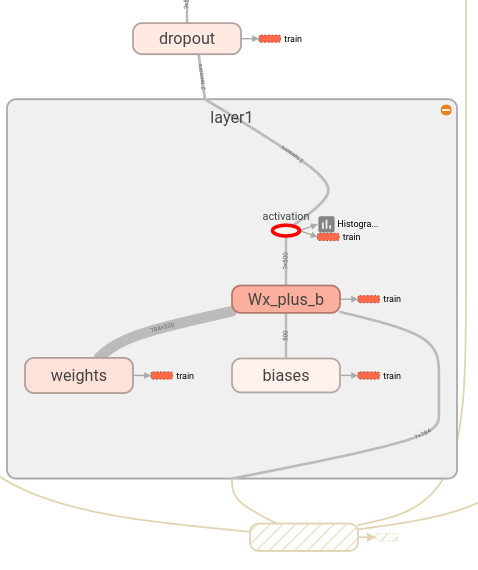
\includegraphics[width=0.45\linewidth,keepaspectratio]{data/chapter-1-1/computing-graph.png}
\caption{模型计算图}
\label{figure:computing-graph}
\end{figure}


在此基础之上,我们在GPU服务器进行模型训练, 依据图 \ref{figure:w2v-loss}所示, 我们可以发现其loss下降很明显。 

\begin{figure}[!htbp]
\centering
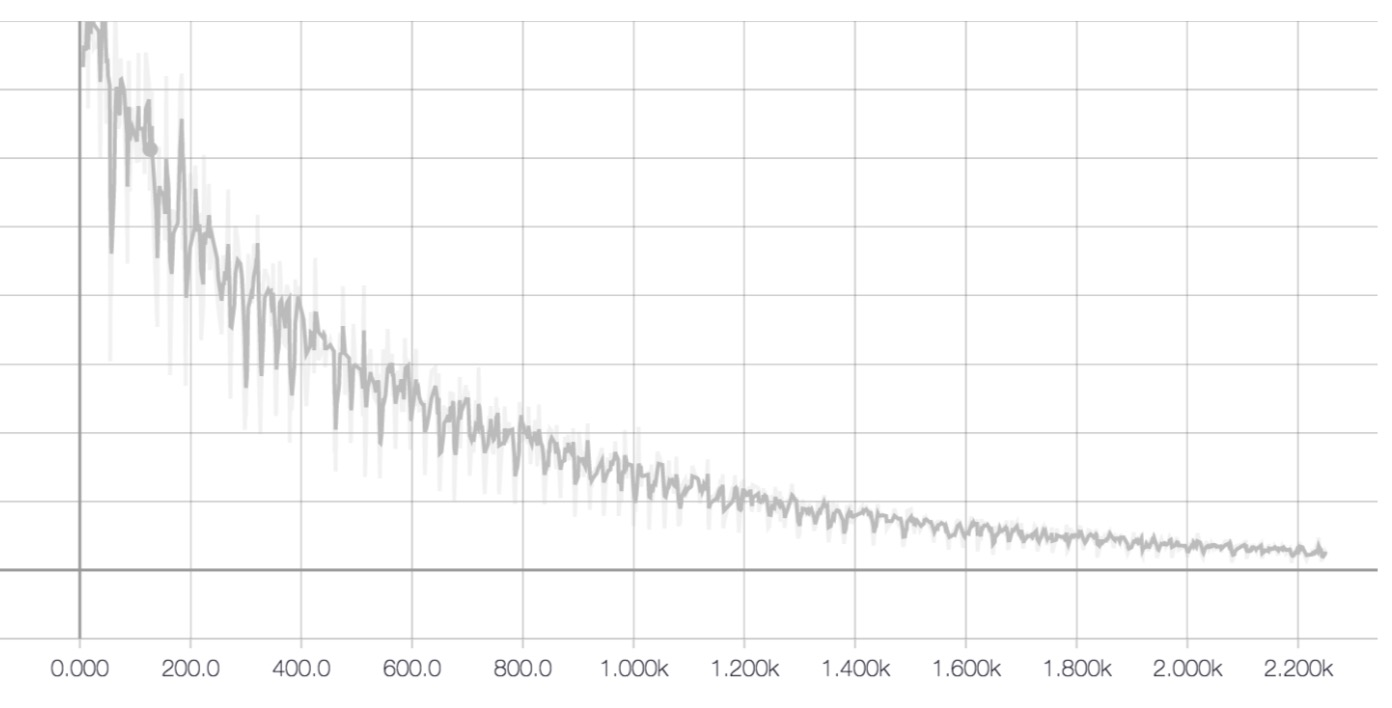
\includegraphics[width=0.45\linewidth,keepaspectratio]{data/chapter-1-1/w2v-loss.png}
\caption{词向量模型loss下降过程}
\label{figure:computing-graph}
\end{figure}

对于该模型来说,在我们限定的词汇大小上(本课题保留的词汇集大小和3万个), 平均每个艺术品描述所包含的词汇经过统计为8个单词, 一共具备43,200条描述信息数据。 则, 对于任意两个单词,判断是否在同一描述信息的准确概率为: 

\begin{equation}
baseline = \frac{C{43200 \choose 1} {8 \choose 1}} {C{43200 \choose 2}} = 0.000185
\end{equation}

基于此基准,则, 如果模型是随机进行判断的, 那么其$loss$值应该为 $-log_2(0.000185) = 12$, 所以如果模型的loss值低于12, 则说明该模型是可以训练的。 实验证明,如图 \ref{eq:art_loss} 模型最终的loss稳定在\textbf{0.1}左右,说明本课题设计的模型可以进行良好的训练。 

\section{本章单词向量化方法的结果分析}

基于以上分析与实验,课题实现了艺术品交易信息的单词向量的训练。 

首先,课题获得的词向量保持了单词的语言相似性,如图 XXX 所示; 


其次, 课题获得的词向量保持了线性计算关系, 如图 XXX 所示;

而且, 课题获得的词向量可以计算单词是否同属一个类型。

词向量具有以上特点, 这表明了单词向量保持语言相似性的良好特性。 该向量为之后句子长度、段落长度的语义分析提供了基础。 

\section{本章小节}

本章通过分析现有单词词向量的方法,说明了使用简单的one-hot与tfidf实现词向量的缺点。 从而使用了更为先进的, 基于深度学习的word2vec方法, word2vec可以良好的保持单词语义级别的相似性。 但是,经过分析,word2vec方法直接应用到本课题的数据是有问题的。 因为本课题的每一条艺术品描述信息都比较短, 这导致使用word2vec模型会缺乏足够的上下分(context words),不能良好的保持语言相似性。课题参加word2vec的基本思想,还参考了Stanford NLP Group 提出的 GloVe, 设计了一种新的词向量方法。 并且在GPU服务器与tensorflow 框架下实现了神经网络结构,实现了词向量的训练。 而且本章还展示了训练得出的词向量在: 1. 同义词判断; 2. 词向量的线性关系; 3.判断语义同属关系。 这三个重要特性的表现, 说明课题训练的词向量良好的保持了语义相似性, 为之后基于更长的自然语义进行语义分析提供了基础。 